%%

In this paper, we have presented context-aware deep network models for WSL. 
Building on recent improvements in region-based CNNs, 
we designed a novel localization architecture integrating the idea of contrast-based contextual guidance to the weakly-supervised object localization. We studied the localization component of a weakly-supervised 
detection network and proposed  a subnetwork that effectively makes use of visual contextual information 
that helps 
refining the boundaries of detected objects.
Our results show that the proposed semantic contrast is an effective cue for obtaining more accurate object 
boundaries. Qualitative results show that our method is less sensitive to the typical failure mode of WSL methods, such as 
shrinking to discriminative object parts. Our method has been validated on VOC 2007 and 2012 benchmarks demonstrating
significant improvements over the baselines.
%%

Given the prohibitive cost of large-scale exhaustive annotation, it is crucial to further develop methods for weakly-supervised visual learning. We believe the proposed approach is complementary to many previously explored ideas and could be combined with other techniques to foster further improvements.
%%



%\def \imgh {1.5cm}
%\def \imgw {1.9cm}

\begin{figure*}
\begin{center}
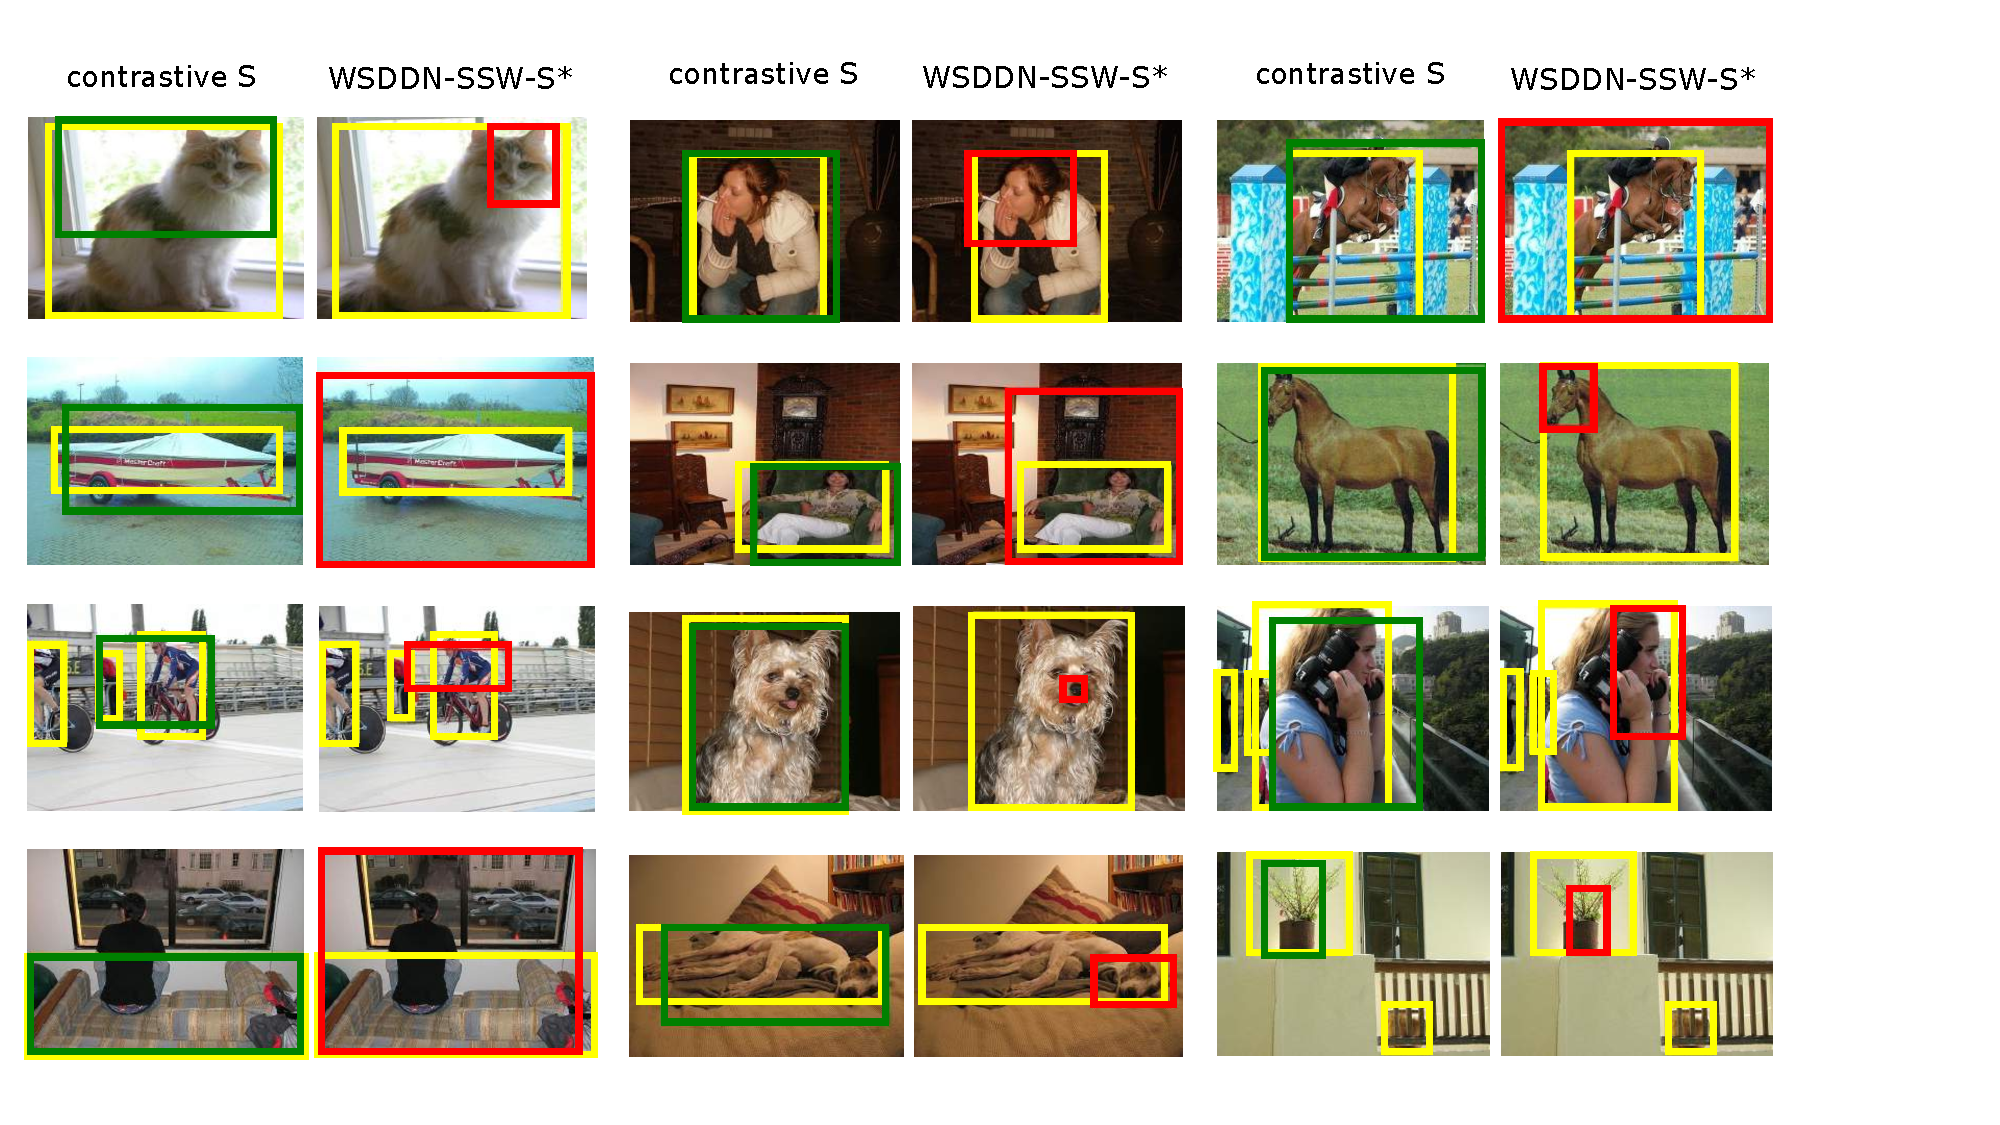
\includegraphics[trim = 0cm 0.8cm 2.8cm 0cm, clip, width=0.98\linewidth] {eccv16_figures/detectionresults_goodbad_1_compressed.pdf}
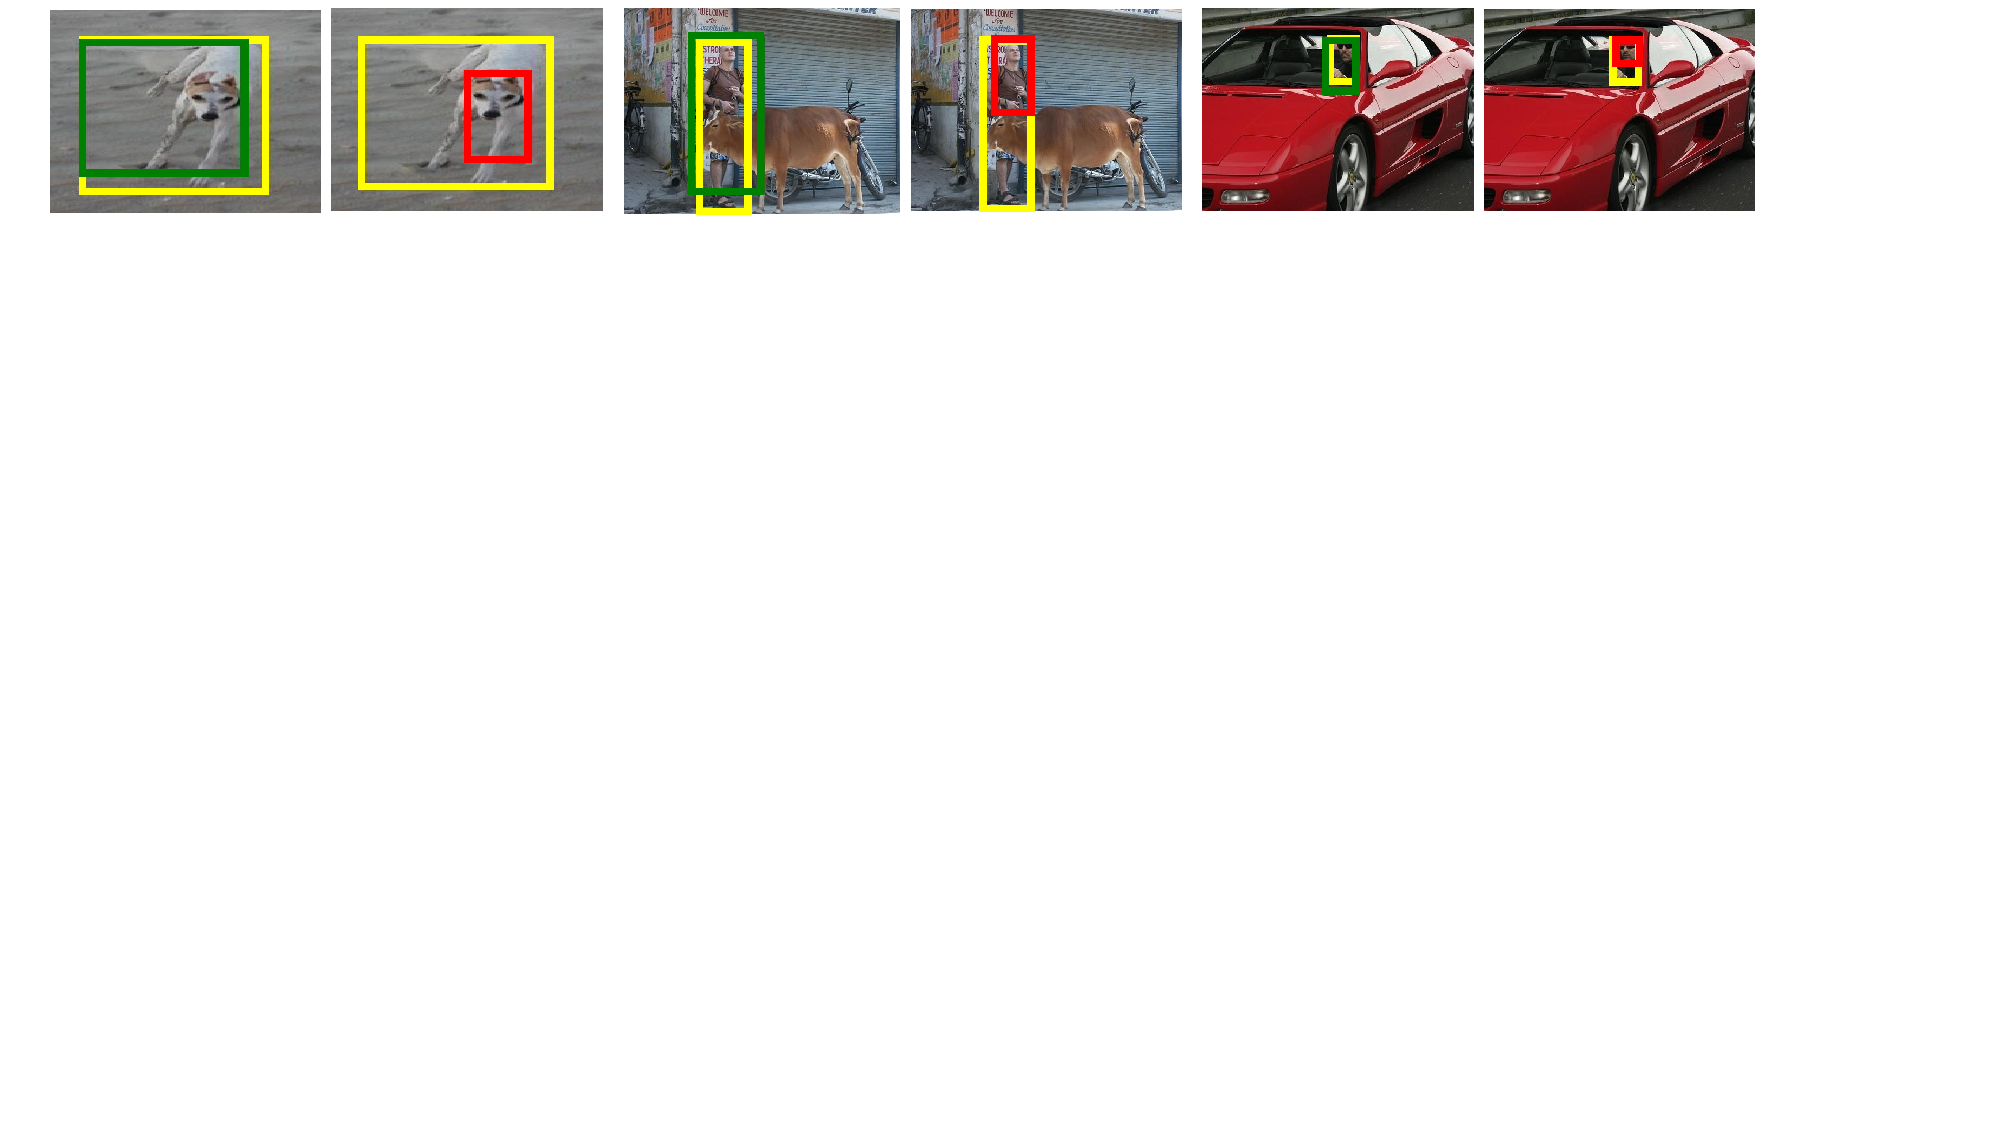
\includegraphics[trim = 0cm 13.5cm 2.8cm 0cm, clip, width=1.0\linewidth] {eccv16_figures/detectionresults_goodbad_4.pdf}
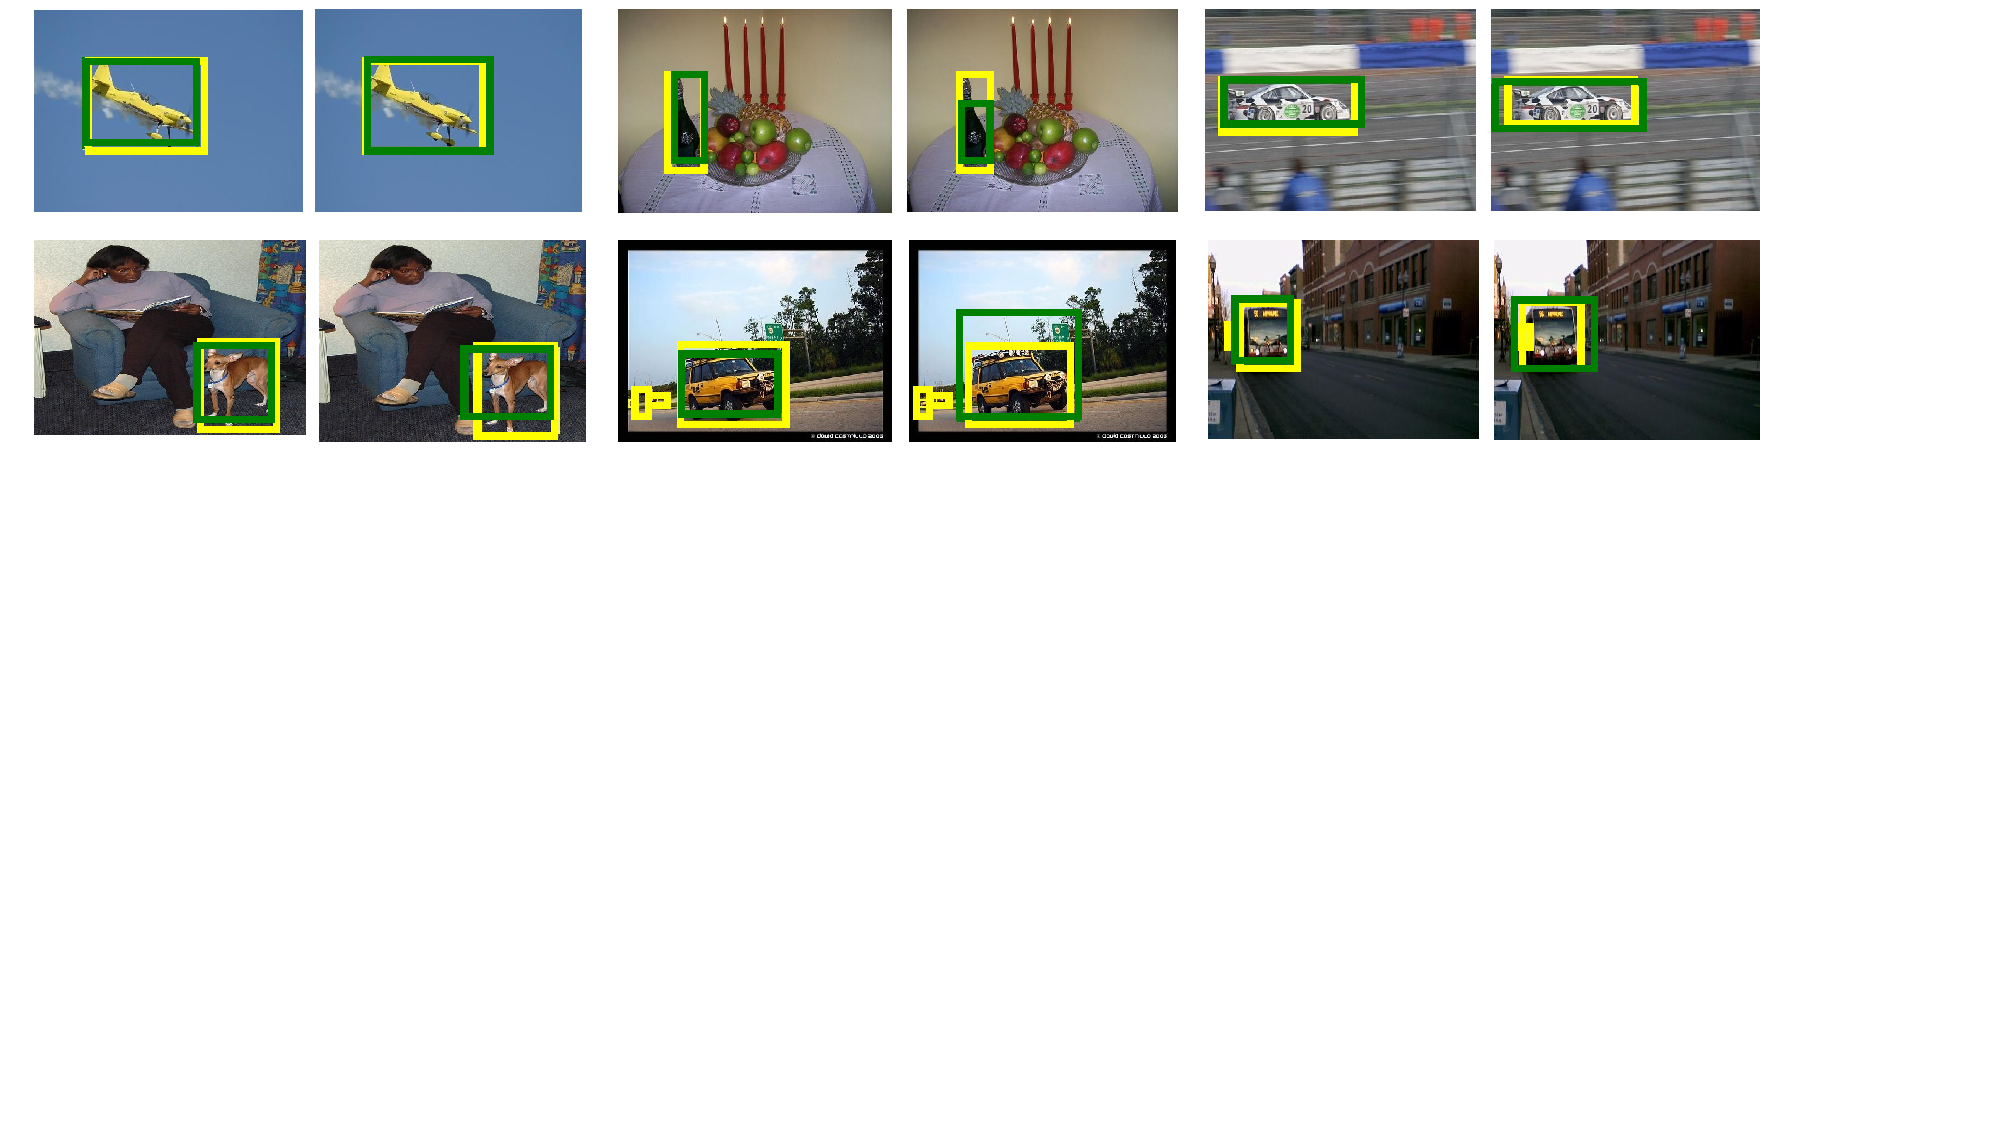
\includegraphics[trim = 0cm 10cm 3cm 0cm, clip, width=0.985\linewidth] {eccv16_figures/detectionresults_goodbad_3.pdf}
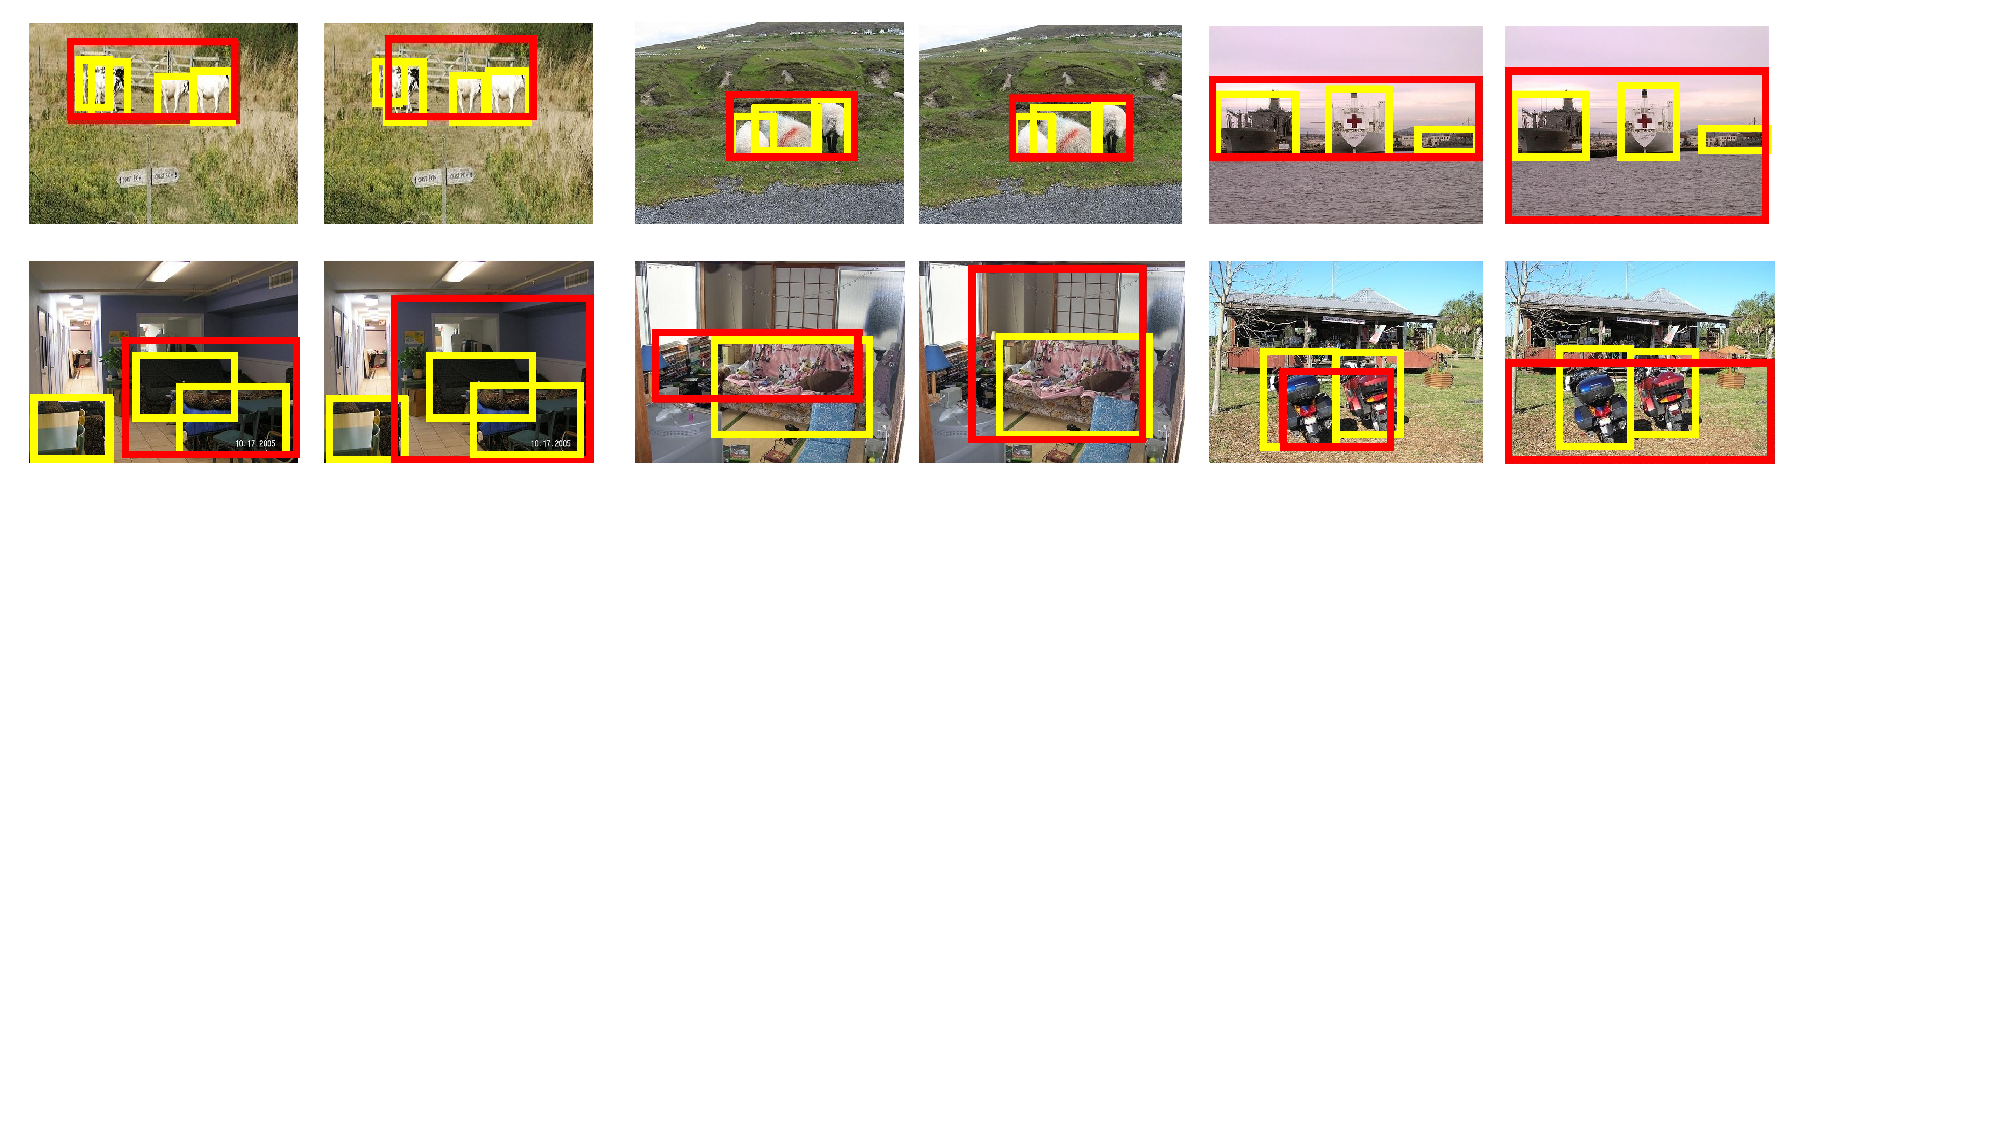
\includegraphics[trim = 0cm 11cm 3cm 0cm, clip, width=0.98\linewidth] {eccv16_figures/detectionresults_goodbad_2.pdf}
\mbox{}\vspace{-.3cm}\\
\end{center}
\caption[Localization examples]{The first five rows show localization examples where our method (contrastive S) outperforms WSDDN-SSW-S$^*$ baseline. Two next rows show examples where both methods succeed. The last two rows illustrate failure cases for both methods. Our method often suceeds in localizing correct object boundaries on examples where WSDNN-SSW-S$^*$ is locked to descriminative object parts such as heads of people and animals. Typical failure cases for both methods include images with multiple objects of the same class.}
\label{fig:detexamples}
\end{figure*}




\subsubsection{Acknowledgments.}
We thank Hakan Bilen, Relja Arandjelovi\'{c}, and Soumith Chintala for fruitful discussion and help.
This work was supported by the ERC grants VideoWorld and Activia, and the MSR-INRIA laboratory.

%%
%%
